\chapter{Flujo Emergente}

En este cap\'itulo se desarrolla la simulaci\'on del modelo de Flujo Emergente, el cu\'al fue considerado dado que algunas observaciones \citep{flux_reference} parecen proveer de evidencia de que los campos magn\'eticos se pueden comportar seg\'un lo descrito por la teor\'ia concerniente. 

\textbf{Escala de altura (h). }Es un valor emp\'irico que permite determinar qu\'e tanto se difumina el campo magn\'etico con respecto a la altura. Su valor fue seleccionado de tal forma que los rangos de sus valores caigan dentro de los emp\'iricos que han sido observados. Concretamente, se tom\'o el valor de 200 debido a que arroja los resultados emp\'iricos observados, que van de 500 a 1000G \citep{VAULT1}.

\textbf{Flujo magn\'etico (phi). }Representa el campo magn\'etico total que pasa por un \'area determinada. Para realizar las pruebas a la extensi\'on computacional propuesta, se tom\'o como valor del flujo magn\'etico $\phi=2.8x10^{18}$Mx. Si bien existe debate sobre las aproximaciones m\'as precisas con respecto a este valor \citep{magneticflux}; se consider\'o \'este debido a que los resultados del radio inicial del tubo de flujo del modelo de Flujo Emergente fueron coherentes con la teor\'ia (366km \citep{magneticflux} y \citep{VAULT2}) al utilizarlo.

\textbf{Intensidad de campo inicial en su base (B0). }Se refiere al valor que toma el campo magn\'etico en la base, o desde el punto donde se desea comenzar a medir. Los c\'alculos fueron generados considerando distintos valores de campo magn\'etico (0, 500, 1000 y 1500 Gauss), dado que en la literatura se ha dado este valor entre 1000 y 1500 Gauss. La fuerza de la red cromosf\'erica es 1 kG a z=0 con una altura de 500km de acuerdo a \citep{judge}.

La representaci\'on geom\'etrica de este modelo puede observarse en la imagen \ref{Flujo_emergente}.

\clearpage
\section{Resultados}

En esta secci\'on se presentar\'an los resultados obtenidos de las simulaciones seg\'un los modelos de arcos magn\'eticos y flujo emergente.

El m\'odelo de Flujo emergente es m\'as complejo que el modelo de arcos magn\'eticos, lo que lo hace f\'isicamente m\'as plausible. Sin embargo, es un modelo que no provee de explanantes a la generaci\'on de los campos magn\'eticos.

Al igual que con el modelo anterior. Primero se calcul\'o el perfil de los campos magn\'eticos seg\'un esta teor\'ia. Para esto, y como se explic\'o en secciones anteriores, se utilizaron los valores de 500, 1000 y 1500G. Como se puede apreciar en la Figura \ref{fe_Campo_Magnetico}, la intensidad del campo magn\'etico decae mucho m\'as r\'apido en comparaci\'on con el modelo anterior, a tal grado que para los 1,000km ya es pr\'acticamente despreciable su valor. Este fen\'omeno es a\'un m\'as acertado a las teor\'ias pertinentes.

Similarmente a lo realizado en el modelo de Flujo emergente, una vez obtenidos los valores del perfil de los campos magn\'eticos se procedi\'o a calcular la presi\'on cromosf\'erica. En este modelo se puede entrever un desplazamiento en la ca\'ida de la presi\'on de la crom\'osfera (V\'ease Figura \ref{fe_Presion}). A su vez, con este nuevo valor, se obtuvo el perfil de densidad, el cual presenta un desplazamiento en el gr\'afico para cada valor de campo. 
Finalmente, una vez obtenidos todos estos resultados, tambi\'en se procedi\'o a realizar dos comparativos entre los resultados de las diferentes perfiles de densidades. Los resultados de estas comparativas se pueden apreciar en la Figura \ref{fe_diferencias_absolutas} y Figura \ref{fe_diferencias_relativas}.

\begin{figure}[h]
\centering
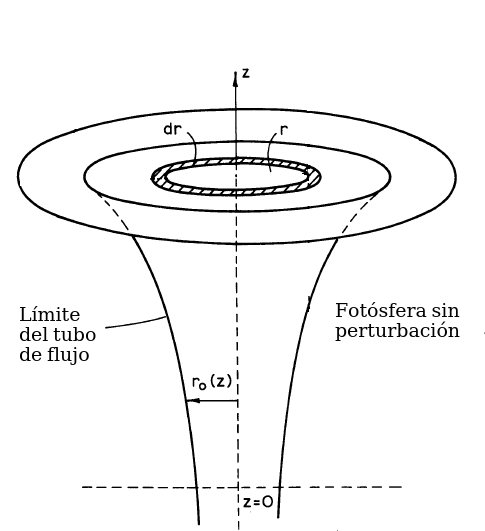
\includegraphics[scale=1]{Flujo_emergente}
\caption{ Representaci\'on geom\'etrica del modelo de flujo emergente. }
\label{Flujo_emergente}
\end{figure}

\begin{figure}[h]
\centering
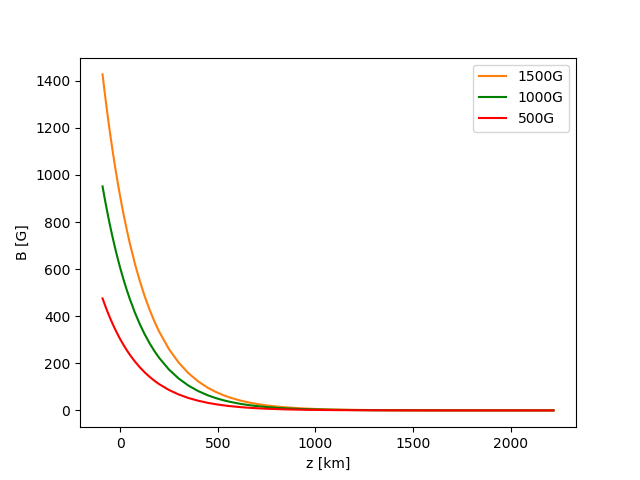
\includegraphics[scale=1]{fe_Campo_Magnetico}
\caption{ En esta gr\'afica se describe el comportamiento de la intensidad del campo magn\'etico. }
\label{fe_Campo_Magnetico}
\end{figure}

\begin{figure}[h]
\centering
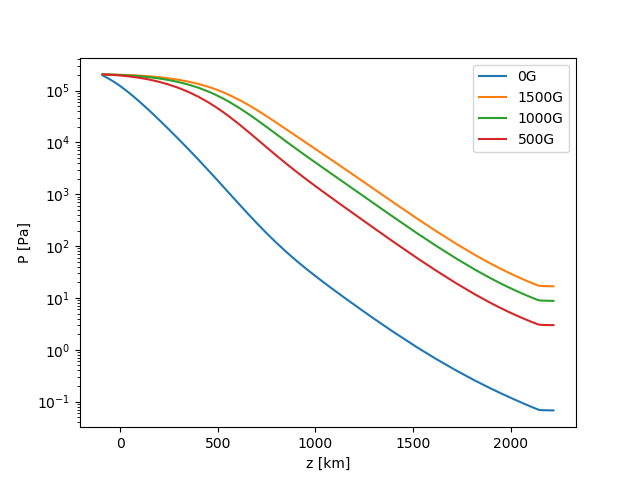
\includegraphics[scale=1]{fe_Presion}
\caption{ Aqu\'i se presentan cada una de las salidas de las simulaciones con los distintos valores de campo magn\'etico seg\'un los resultados anteriores.}
\label{fe_Presion}
\end{figure}

\begin{figure}[h]
\centering
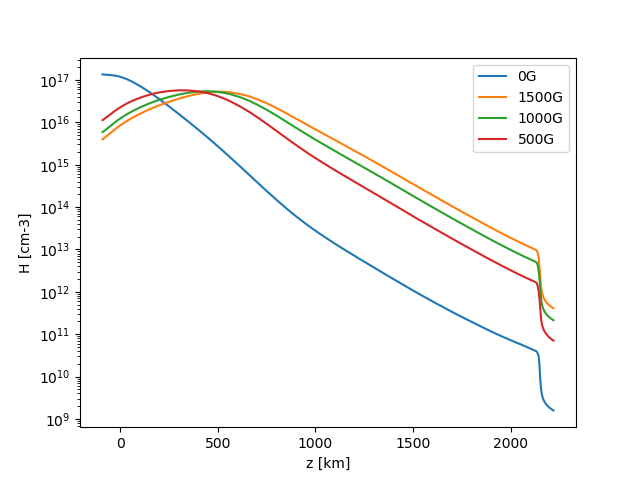
\includegraphics[scale=1]{fe_perfil_de_densidades}
\caption{ En esta figura se grafican el perfil de densidades de hidr\'ogeno.}
\label{fe_perfil_de_densidades}
\end{figure}


\begin{figure}[h]
\centering
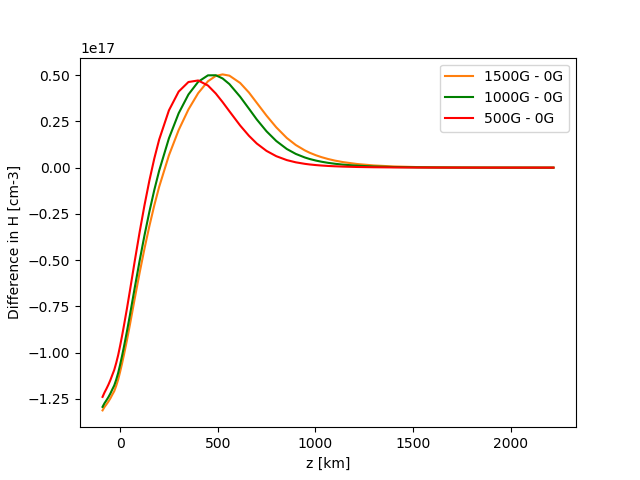
\includegraphics[scale=1]{fe_diferencias_absolutas}
\caption{ Aqu\'i se muestra una comparaci\'on entre las diferentes salidas de las densidades del programa.}
\label{fe_diferencias_absolutas}
\end{figure}

\begin{figure}[h]
\centering
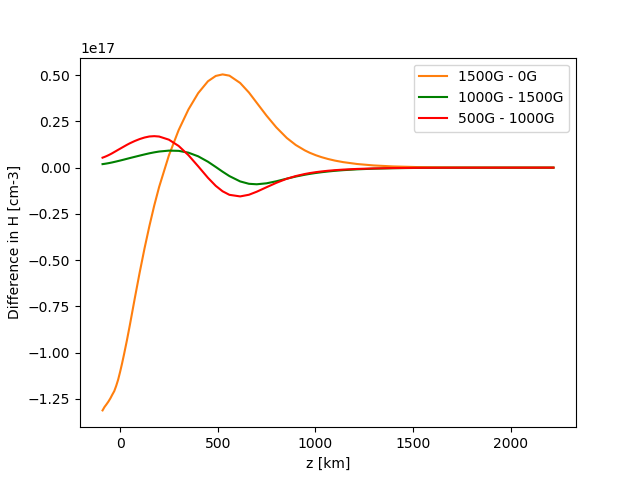
\includegraphics[scale=1]{fe_diferencias_relativas}
\caption{ Aqu\'i se muestra un diferencial de cada uno de las salidas de las simulaciones contra las salidas de la simulaci\'on con un valor m\'as bajo.}
\label{fe_diferencias_relativas}
\end{figure}
